% Options for packages loaded elsewhere
\PassOptionsToPackage{unicode}{hyperref}
\PassOptionsToPackage{hyphens}{url}
\documentclass[
]{article}
\usepackage{xcolor}
\usepackage[margin=1in]{geometry}
\usepackage{amsmath,amssymb}
\setcounter{secnumdepth}{5}
\usepackage{iftex}
\ifPDFTeX
  \usepackage[T1]{fontenc}
  \usepackage[utf8]{inputenc}
  \usepackage{textcomp} % provide euro and other symbols
\else % if luatex or xetex
  \usepackage{unicode-math} % this also loads fontspec
  \defaultfontfeatures{Scale=MatchLowercase}
  \defaultfontfeatures[\rmfamily]{Ligatures=TeX,Scale=1}
\fi
\usepackage{lmodern}
\ifPDFTeX\else
  % xetex/luatex font selection
\fi
% Use upquote if available, for straight quotes in verbatim environments
\IfFileExists{upquote.sty}{\usepackage{upquote}}{}
\IfFileExists{microtype.sty}{% use microtype if available
  \usepackage[]{microtype}
  \UseMicrotypeSet[protrusion]{basicmath} % disable protrusion for tt fonts
}{}
\makeatletter
\@ifundefined{KOMAClassName}{% if non-KOMA class
  \IfFileExists{parskip.sty}{%
    \usepackage{parskip}
  }{% else
    \setlength{\parindent}{0pt}
    \setlength{\parskip}{6pt plus 2pt minus 1pt}}
}{% if KOMA class
  \KOMAoptions{parskip=half}}
\makeatother
\usepackage{longtable,booktabs,array}
\usepackage{calc} % for calculating minipage widths
% Correct order of tables after \paragraph or \subparagraph
\usepackage{etoolbox}
\makeatletter
\patchcmd\longtable{\par}{\if@noskipsec\mbox{}\fi\par}{}{}
\makeatother
% Allow footnotes in longtable head/foot
\IfFileExists{footnotehyper.sty}{\usepackage{footnotehyper}}{\usepackage{footnote}}
\makesavenoteenv{longtable}
\usepackage{graphicx}
\makeatletter
\newsavebox\pandoc@box
\newcommand*\pandocbounded[1]{% scales image to fit in text height/width
  \sbox\pandoc@box{#1}%
  \Gscale@div\@tempa{\textheight}{\dimexpr\ht\pandoc@box+\dp\pandoc@box\relax}%
  \Gscale@div\@tempb{\linewidth}{\wd\pandoc@box}%
  \ifdim\@tempb\p@<\@tempa\p@\let\@tempa\@tempb\fi% select the smaller of both
  \ifdim\@tempa\p@<\p@\scalebox{\@tempa}{\usebox\pandoc@box}%
  \else\usebox{\pandoc@box}%
  \fi%
}
% Set default figure placement to htbp
\def\fps@figure{htbp}
\makeatother
% definitions for citeproc citations
\NewDocumentCommand\citeproctext{}{}
\NewDocumentCommand\citeproc{mm}{%
  \begingroup\def\citeproctext{#2}\cite{#1}\endgroup}
\makeatletter
 % allow citations to break across lines
 \let\@cite@ofmt\@firstofone
 % avoid brackets around text for \cite:
 \def\@biblabel#1{}
 \def\@cite#1#2{{#1\if@tempswa , #2\fi}}
\makeatother
\newlength{\cslhangindent}
\setlength{\cslhangindent}{1.5em}
\newlength{\csllabelwidth}
\setlength{\csllabelwidth}{3em}
\newenvironment{CSLReferences}[2] % #1 hanging-indent, #2 entry-spacing
 {\begin{list}{}{%
  \setlength{\itemindent}{0pt}
  \setlength{\leftmargin}{0pt}
  \setlength{\parsep}{0pt}
  % turn on hanging indent if param 1 is 1
  \ifodd #1
   \setlength{\leftmargin}{\cslhangindent}
   \setlength{\itemindent}{-1\cslhangindent}
  \fi
  % set entry spacing
  \setlength{\itemsep}{#2\baselineskip}}}
 {\end{list}}
\usepackage{calc}
\newcommand{\CSLBlock}[1]{\hfill\break\parbox[t]{\linewidth}{\strut\ignorespaces#1\strut}}
\newcommand{\CSLLeftMargin}[1]{\parbox[t]{\csllabelwidth}{\strut#1\strut}}
\newcommand{\CSLRightInline}[1]{\parbox[t]{\linewidth - \csllabelwidth}{\strut#1\strut}}
\newcommand{\CSLIndent}[1]{\hspace{\cslhangindent}#1}
\setlength{\emergencystretch}{3em} % prevent overfull lines
\providecommand{\tightlist}{%
  \setlength{\itemsep}{0pt}\setlength{\parskip}{0pt}}
\usepackage{float} \floatplacement{figure}{H}
\usepackage{subfig}
\usepackage{booktabs}
\usepackage{longtable}
\usepackage{array}
\usepackage{multirow}
\usepackage{wrapfig}
\usepackage{float}
\usepackage{colortbl}
\usepackage{pdflscape}
\usepackage{tabu}
\usepackage{threeparttable}
\usepackage{threeparttablex}
\usepackage[normalem]{ulem}
\usepackage{makecell}
\usepackage{xcolor}
\usepackage{bookmark}
\IfFileExists{xurl.sty}{\usepackage{xurl}}{} % add URL line breaks if available
\urlstyle{same}
\hypersetup{
  pdftitle={On the use of difference and ratio scores in sleep discrepancy research},
  pdfauthor={Tom F. Walton1; Melissa J. Ree1; Romola S. Bucks1,2,3},
  hidelinks,
  pdfcreator={LaTeX via pandoc}}

\title{On the use of difference and ratio scores in sleep discrepancy research}
\author{Tom F. Walton\textsuperscript{1} \and Melissa J. Ree\textsuperscript{1} \and Romola S. Bucks\textsuperscript{1,2,3}}
\date{2023-09-04}

\begin{document}
\maketitle

\textsuperscript{1} School of Psychological Science, The University of Western Australia\\
\textsuperscript{2} School of Population and Global Health, The University of Western Australia\\
\textsuperscript{3} Office of the Deputy Vice Chancellor, Research, The University of Western Australia

\section{Abstract}\label{abstract}

\subsection{Introduction}\label{introduction}

The discordance that can exist between objective and self-report measures of sleep is known as sleep discrepancy. Sleep discrepancy is an important feature of insomnia disorder and a central issue in the measurement of sleep. In studies exploring the relationship between sleep discrepancy and other variables of interest, discrepancy is almost always operationalised with a derived index, such as a difference score formed by subtracting self-report sleep objective sleep. Substantial problems with derived indices have been emphasised by a number of authors. We aimed to investigate and demonstrate these problems in the context of sleep discrepancy.

\subsection{Method}\label{method}

Archival data from the Healthy Ageing Research Programme, a longitudinal study investigating cognition in older adults, were used to provide empirical demonstrations of problems with derived indices. Objective sleep was recorded from 297 participants using actigraphy with concurrent sleep diaries. Participants also completed a range of questionnaires including the insomnia severity index.

\subsection{Results}\label{results}

Derived indices were associated with the following problems (i) directionality: the full range of the discrepancy variable can be neglected when characterising a discrepancy effect and (ii) implicit coefficient weights: derived indices impose constraints on relationships with outcome variables that are untested and often theoretically inappropriate. Model comparisons using multiple, constrained, piece-wise, and moderated regressions indicated that assumptions represented by the aforementioned problems were not supported by the data. Moreover, a relationship of sleep discrepancy to insomnia symptom severity, apparent with traditional approaches, was not observed following closer investigation with more appropriate procedures.

\subsection{Conclusion}\label{conclusion}

The use of derived indices in sleep discrepancy research is associated with substantial conceptual and methodological problems, such that findings from studies incorporating derived scores into subsequent statistical analyses may be spurious. Accurate testing for discrepancy effects is a task considerably more complicated than it initially appears. In the future, study designs should be modified or alternative analytic approaches should be employed such as response surface analysis, spline regression, or latent difference score modelling.

\section{Introduction}\label{introduction-1}

Sleep discrepancy, sometimes referred to as subjective-objective sleep discrepancy or sleep misperception, is the discordance between self-report and objective measures of sleep. Sleep discrepancy can be considered a spectrum ranging from negative (where self-report sleep exceeds objective sleep) to positive (where objective sleep exceeds self-report sleep). Negative sleep discrepancy is commonly observed in insomnia, where measures such as total sleep time (TST) and wake after sleep onset (WASO) tend to be under-and overestimated by affected individuals, respectively, in comparison with objective recordings (Edinger \& Fins, 1995; Manconi et al., 2010; \textbf{fernandez-mendoza2011?}). This phenomenon plays a central role in many theories of insomnia. For example, individuals who underestimate their sleep may spend more time in bed to compensate for this perceived lack, increasing sleep fragmentation (as the homoeostatic drive for sleep remains constant), and subsequently anxiety and arousal at sleep (\textbf{harvey2002?}). Positive sleep discrepancy has been less investigated although healthy adults can modestly overestimate their sleep (Mercer et al., 2002) and positive sleep discrepancy in its more extreme forms may be related to dementia (Most et al., 2012).

Many past studies have aimed to investigate the relationship of sleep discrepancy with another construct. This is most commonly achieved by deriving an index such as a difference score (e.g., self-report TST -- objective TST) and adding this as a dependent or independent variable in linear regression-based analyses (Chapter 2; Walton et al., 2025). Whilst this is a convenient strategy with intuitive appeal, the use of derived indices in such a way is associated with a range of conceptual and methodological problems (Chapter 3; Cronbach \& Furby, 1970; Edwards, 1994; Griffin et al., 1999; Kronmal, 1993; \textbf{wittenborn1951?}). These problems are substantive and inferences made on the basis of derived indices may be misleading or incorrect. Using real sleep data, we provide an in-depth treatment of problems with derived indices in the context of sleep discrepancy research. The following section describes the data and and methods for its collection. We then introduce derived indices and enumerate the specific problems associated with each. Finally, we explore alternative strategies that can be employed to address the issues posed by derived indices.

\section{Data and methods}\label{data-and-methods}

Data for empirical demonstrations were obtained from the Healthy Ageing Research Program, a longitudinal study of cognition in ageing, based in Perth, Western Australia. Community-dwelling older adults (N = 230; aged 50+) completed cognitive testing, clinical and demographic questionnaires, and a week of sleep measurement between 2014 to 2018. Objective sleep was recorded with Actigraphy (Tri-axial wGT3X-BT activity monitor; Actigraph LLC, Pensacola, FL). Scoring was performed with the Cole-Kripke algorithm in Acti-life software (version 6.11.8) using 60-second epochs. Estimates of TST were provided automatically by the software. Self-report sleep was measured with the Consensus Sleep Diary (CSD; Carney et al., 2012). Estimates of self-report TST were calculated by subtracting wake after sleep onset (WASO) and sleep onset latency (SOL) from sleep period time (SPT). SPT was defined as the length of time between a participant's bedtime and their final awakening. The Insomnia Severity Index (ISI; \textbf{bastien2001?}) was used as an outcome variable for all empirical demonstrations. The ISI is a 7-item scale querying the presence of insomnia symptoms over the past 2-week period and was administered prior to sleep measurements alongside a range of other questionnaires. The study was approved by the UWA Human Research Ethics Committee (RA/4/1/536).

Note there are some methodological considerations for this data that affect its suitability for scientific inference. Consequently findings should be interpreted as demonstrations only. Firstly, data were aggregated across nights and testing visits, ignoring the correlation of errors within individuals. Standard errors will be underestimated as a result and statistical power will be affected. As the demonstrations compare different statistical approaches to the same data, this is not expected to affect the strength of our conclusions. Secondly, actigraphy bed and rise times were defined using diary estimates of the same, with highly discrepant (\textgreater60 minute) sleep periods inspected and scored visually according to the Society of Behavioural Sleep Medicine (SBSM; Ancoli-Israel et al., 2015). Using self-report measures for definition of objective sleep parameters is inappropriate for sleep discrepancy research and artificially reduces the discordance between self-report and objective measures (Chapter 2; Walton et al., 2025).

This manuscript, including all statistical analyses, tables, and figures was generated using computationally reproducible methods (Lindsay, 2023; Piccolo \& Frampton, 2016) in R version 4.4.2 (2024-10-31 ucrt) (R Core Team, 2023) with R Studio (Posit team, 2024) and R Markdown (Allaire et al., 2023). Packages included tidyverse (Wickham et al., 2019), bookdown (Xie, 2023a), knitr (Xie, 2023b), kableExtra (Zhu, 2023), restriktor (Vanbrabant \& Kuiper, 2023), segmented (Muggeo, 2008), ggplot2 (\textbf{wickham2016?}), and DiagrammeR (Iannone, 2023). Code is available through the Github repository \url{https://github.com/tfwalton/sleep-discrepancy-methods}.

\section{Introduction to derived indices}\label{introduction-to-derived-indices}

There are three principal categories of quantitative sleep discrepancy indices: difference scores, ratio scores, and combination scores that incorporate both differences and ratios. A simple algebraic difference score, such as that formed by subtracting self-report total sleep time (TST) from objective TST, is the most common sleep discrepancy index (Chapter 2; Walton et al., 2025)

\begin{equation}
dTST = sTST - oTST
\label{eq:dTST}
\end{equation}

Here, positive sleep discrepancy is represented by positive values and negative discrepancy by negative values. For algebraic difference scores such as dTST, objective sleep will most commonly feature as the variable that is subtracted from the other (i.e., the minuend) however there are cases where the subtraction is reversed and the direction of the difference score is switched.

Absolute difference scores are also sometimes used such as the following:

\begin{equation}
absTST = |sTST - oTST|
\label{eq:absTST}
\end{equation}

Unlike simple algebraic difference scores, absolute difference scores operationalise positive and negative discrepancy as the same quantity.

The most common ratio score used in sleep discrepancy research is that formed by the division of sTST by oTST, expressed as a percentage (Chapter 2; Walton et al., 2025):

\begin{equation}
rTST = \frac{sTST}{oTST}*100
\label{eq:rTST}
\end{equation}

This index is also known as objective sleep time estimated (OSE) and was introduced by Edinger \& Fins (1995) in their seminal paper. For rTST, values over and under 100 indicate positive and negative discrepancy, respectively. Ratio scores typically feature objective sleep as the denominator, however, as with algebraic difference scores, this is sometimes reversed. For simplicity, ratio scores will be expressed as proportions rather than percentages for the remainder of the paper.

The most common combination score is the misperception index (MI) developed by Manconi et al. (2010), defined as:

\begin{equation}
MI = \frac{oTST-sTST}{oTST}
\label{eq:MI}
\end{equation}

The MI was constructed to reproduce the bimodal distribution observed with OSE in insomnia patients whilst providing a strong correspondence to the difference score oTST-sTST. Possible values for the MI range from \(-\infty\) (extreme over-estimation) to +1 (extreme underestimation), although Manconi et al. (2010) recommends trimming the lower limit to -1.

The features and initial differences between these four quantitative indices can be illustrated by generating some example values of sTST and oTST and observing the resulting index values (see Table \ref{tab:samples})

\begin{table}[!h]
\centering
\caption{\label{tab:samples}Comparison of Quantitative Indices}
\centering
\fontsize{10}{12}\selectfont
\begin{threeparttable}
\begin{tabular}[t]{>{\raggedleft\arraybackslash}p{2em}>{\raggedleft\arraybackslash}p{2em}>{\raggedright\arraybackslash}p{5em}>{\raggedleft\arraybackslash}p{2em}>{\raggedleft\arraybackslash}p{4em}>{\raggedright\arraybackslash}p{2em}>{\raggedright\arraybackslash}p{3em}>{\raggedright\arraybackslash}p{2em}>{\raggedright\arraybackslash}p{3em}>{\raggedright\arraybackslash}p{2em}>{\raggedright\arraybackslash}p{3em}>{\raggedright\arraybackslash}p{2em}}
\toprule
sTST & oTST & Category & dTST & absTST &  & rTST &  & 1/rTST &  & MI & \\
\midrule
200 & 100 & Positive & 100 & 100 & \textcolor{gray}{\raisebox{-5mm}{50}} & 2 & \textcolor{gray}{\raisebox{-5mm}{\hspace{-5mm}0.75}} & 0.5 & \textcolor{gray}{\raisebox{-5mm}{\hspace{-5mm}0.3}} & -1 & \textcolor{gray}{\raisebox{-5mm}{\hspace{-5mm}0.75}}\\
\addlinespace
250 & 200 & Positive & 50 & 50 & \textcolor{gray}{\raisebox{-5mm}{50}} & 1.25 & \textcolor{gray}{\raisebox{-5mm}{\hspace{-5mm}0.25}} & 0.8 & \textcolor{gray}{\raisebox{-5mm}{\hspace{-5mm}0.2}} & -0.25 & \textcolor{gray}{\raisebox{-5mm}{\hspace{-5mm}0.25}}\\
\addlinespace
300 & 300 & No discrepancy & 0 & 0 & \textcolor{gray}{\raisebox{-5mm}{50}} & 1 & \textcolor{gray}{\raisebox{-5mm}{\hspace{-5mm}0.125}} & 1 & \textcolor{gray}{\raisebox{-5mm}{\hspace{-5mm}0.143}} & 0 & \textcolor{gray}{\raisebox{-5mm}{\hspace{-5mm}0.125}}\\
\addlinespace
350 & 400 & Negative & -50 & 50 & \textcolor{gray}{\raisebox{-5mm}{50}} & 0.875 & \textcolor{gray}{\raisebox{-5mm}{\hspace{-5mm}0.075}} & 1.14 & \textcolor{gray}{\raisebox{-5mm}{\hspace{-5mm}0.107}} & 0.125 & \textcolor{gray}{\raisebox{-5mm}{\hspace{-5mm}0.075}}\\
\addlinespace
400 & 500 & Negative & -100 & 100 & \textcolor{gray}{\raisebox{-5mm}{}} & 0.8 & \textcolor{gray}{\raisebox{-5mm}{\hspace{-5mm}}} & 1.25 & \textcolor{gray}{\raisebox{-5mm}{\hspace{-5mm}}} & 0.2 & \textcolor{gray}{\raisebox{-5mm}{\hspace{-5mm}}}\\
\addlinespace
\bottomrule
\end{tabular}
\begin{tablenotes}[para]
\item \textit{Note: } 
\item oTST = objective TST, sTST = self-report TST, dTST = sTST - oTST, absTST = |sTST-oTST|, rTST = (sTST/oTST)*100, 1/rTST = 1/(sTST/oTST)*100, MI = misperception index, the absolute values of differences between consecutive rows for each quantitative index are offset to the right in grey.
\end{tablenotes}
\end{threeparttable}
\end{table}

Whilst the magnitudes of the differences between consecutive rows of algebraic (dTST) and absolute difference (absTST) scores remain equal, the differences between consecutive ratio and combination scores decrease with increasing magnitudes of self-report and objective sleep. This feature of ratio (rTST, 1/rTST) and combination scores (MI) is akin to a data transformation and its consequences will be discussed in a later paragraph on ratio scores. The misperception index incorporates features from both difference and ratio scores. Whilst the differences between consecutive values are equal in magnitude to those of rTST, the MI has a defined zero-point and a valence that represents direction of discrepancy (although in the opposite direction to dTST). Problems with each variant of derived index are demonstrated in the forthcoming paragraphs. An individual treatment of combination scores will not be provided, as by the end of the section we believe the reader will be satisfied that combination scores inherit all problems associated with their simpler analogues.

\section{Problems with derived indices}\label{problems-with-derived-indices}

\subsection{Simple algebraic difference scores}\label{simple-algebraic-difference-scores}

\subsubsection{Directionality}\label{directionality}

Difference scores operationalise sleep discrepancy as a spectrum in one-dimensional space where negative or positive sleep discrepancy are represented by lower or higher numbers, respectively (see Table \ref{tab:samples}). Often, however, negative sleep discrepancy is theoretically distinct to positive sleep discrepancy with respect to its relationship with another construct. In other words, it usually means something different to overestimate sleep more than to underestimate sleep less. Suppose that a researcher was interested in measuring the correlation between insomnia symptom severity measured by an instrument such as the ISI, and sleep discrepancy as operationalised by the difference score dTST. A correlation coefficient r = .5 could equally represent a case where reduced positive sleep discrepancy corresponds with greater insomnia as one where increased negative sleep discrepancy corresponds with greater insomnia. Most sleep discrepancy research has been focussed on sleep underestimation as a phenomenon (Trajanovic et al., 2007) and the fact that an identified effect exists through the full range of a difference score is often neglected.

There have been some acknowledgements of the issues with directionality implicit in the strategies used for analysis in the literature. For example, Lubas et al. (2022) used clinical measures of the late effects of childhood cancer to predict simple algebraic difference scores in TST, SOL, and SE separately for those with negative and positive sleep discrepancy. This was performed additionally to an analysis of the same predictors and absolute difference scores of the same sleep variables. The viability and implications of strategies such as these are considered later.

We can demonstrate the directionality problem, in isolation of other problems, empirically by using linear and piece-wise regression to predict insomnia severity index (ISI) scores from dTST in the HARP sample. First, the number of sleep underestimators and overestimators can be explored in the data set by calculating the difference score (dTST = actigraphic TST -- diary TST) and plotting a histogram (see Figure \ref{fig:histogram}).

\begin{figure}

{\centering 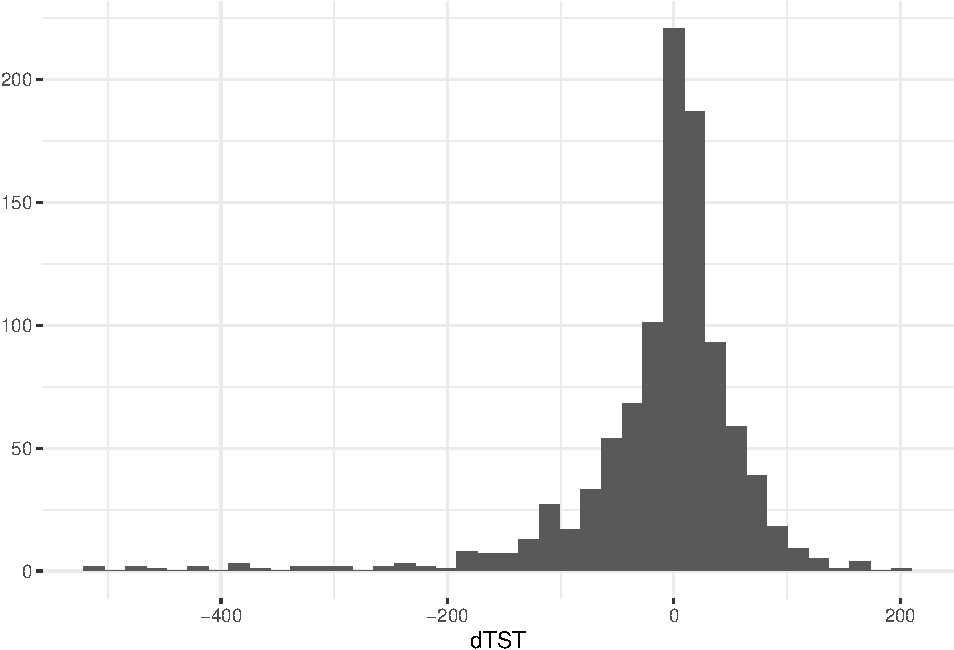
\includegraphics[width=0.8\linewidth]{methods_paper_files/figure-latex/histogram-1} 

}

\caption{Histogram of dTST in sample (N = 997)}\label{fig:histogram}
\end{figure}

Although data are skewed to the left (skewness =-2.33) there appear to be roughly equal proportions of cases exhibiting negative and positive sleep discrepancy. Excluding cases where dTST is equal to exactly zero, approximately 41\% of cases are over and 35\% are under estimators. There is, therefore, a substantial amount of positive discrepancy present in this sample and it is very likely that values on this side of the zero will contribute to any relationship defined by dTST. An approach similar to Lubas et al. (2022) could be performed where the sample is split at 0 into groups of under estimators and over estimators, with separate regressions conducted on each group. However, the decision for where along dTST to split the sample represents another assumption that may not be borne out by the data. For instance, insomnia severity could potentially be minimised at dTST = -30 or dTST = +30, corresponding to modest sleep underestimation and overestimation, respectively. The location of this point along dTST is itself an interesting theoretical question and should be represented as a hypothesis to be tested rather than an assumption implicit in the analysis process.

Whether the relationship of dTST to ISI changes at zero, or another value of dTST, can be tested explicitly by comparing a simple bivariate regression of ISI on dTST, with a piece-wise regression allowing the linear relationship to change at a ``break-point'' along dTST, identified through iterative procedures developed by Muggeo (2003a). Here, we use the ``segmented'' package available for R (Muggeo, 2003b).

First the hypothesis for the existence of a break-point can be tested. Muggeo's score test for one or two changes in the slope of regression (Muggeo, 2016) is statistically significant, \emph{observed value} = 2.03, \emph{p} = .043, indicating that the linear relationship between dTST and ISI changes somewhere along the range of dTST. The parameter estimates for a simple difference score regression of ISI scores on dTST and a corresponding piecewise regression are available in Table \ref{tab:segmented2}. The break-point for the piecewise regression was estimated with a starting value of \(\psi\) = 0.

\begin{table}[!h]
\centering
\caption{\label{tab:segmented2}Regression with difference score and segmented difference score models}
\centering
\fontsize{10}{12}\selectfont
\begin{threeparttable}
\begin{tabular}[t]{>{\raggedright\arraybackslash}p{8em}>{\raggedright\arraybackslash}p{4em}>{\raggedright\arraybackslash}p{8em}>{\raggedright\arraybackslash}p{5em}>{\raggedright\arraybackslash}p{5em}>{\raggedright\arraybackslash}p{5em}}
\toprule
  & Estimate & 95\% CI [LL, UL] & Standard Error & t-value & p-value\\
\midrule
\addlinespace[0.3em]
\multicolumn{6}{l}{\textbf{Linear regression}}\\
\hspace{1em}Intercept & 6.28 & {}[6.03 , 6.54] & 0.13 & 48.2 & < .001\\
\addlinespace
\hspace{1em}dTST & -0.01 & {}[-0.014 , -0.007] & 0.002 & -5.76 & < .001\\
\addlinespace
\addlinespace[0.3em]
\multicolumn{6}{l}{\textbf{Piecewise regression}}\\
\hspace{1em}Intercept & 6.08 & {}[5.79 , 6.36] & 0.145 & 42 & < .001\\
\addlinespace
\hspace{1em}dTST & -0.014 & {}[-0.018 , -0.01] & 0.002 & -6.99 & < .001\\
\addlinespace
\hspace{1em}U1 dTST & 0.043 & {}[0.021 , 0.065] & 0.011 & 3.76 & < .001\\
\addlinespace
\hspace{1em}Break-point & 45.2 & {}[21 , 69.4] & NA & NA & \\
\addlinespace
\bottomrule
\end{tabular}
\begin{tablenotes}[para]
\item \textit{Note: } 
\item CI = confidence intervals, U1 refers to the differences-in-slope coefficient, LL = lower limit, UL = upper limit, dTST = difference score of sTST -- oTST
\end{tablenotes}
\end{threeparttable}
\end{table}

The piecewise regression estimates for the slopes to the left and right of the breakpoint were -0.014 and 0.029, respectively, indicating that the negative association between insomnia severity and dTST becomes positive at approximately 45 minutes of overestimated sleep. Taken together, these results indicate that a segmented relationship is a better explanation for the data than a strictly linear one with the effect of dTST changes direction when self-reported sleep exceeds objective sleep by a given amount.

\subsubsection{Implicit weighting of difference score components}\label{implicit-weighting-of-difference-score-components}

The second major problem with difference scores is less obvious though just as critical. Difference scores hold implicit weightings on the contributions of their component variables to observed relationships, that (i) rarely make theoretical sense and, (ii) often reduce the variance in predicted values that can be accounted for by a model (Edwards, 2002).

Expansion of the dTST term in the regession of predicted ISI values provides

\begin{equation}
ISI = b_{0}+b_{1}({sTST-oTST}) + \epsilon
\label{eq:lmdiff2}
\end{equation}

Expansion of the bracketed terms results in

\begin{equation}
= b_{0} + b_{1} sTST - b_{1}oTST + \epsilon
\label{eq:lmdiff3}
\end{equation}

From the above, we can observe that a regression of difference score dTST is equivalent to a multiple regression of sTST and oTST where the regression coefficients for each term are constrained to be equal but opposite in magnitude. These constraints can be made more explicit by factoring (Edwards, 2002):

\begin{equation}
= b_{0} + (1)b_{1}sTST + (-1)b_{1}oTST + \epsilon
\label{eq:lmdiff4}
\end{equation}

In this example, for the prediction of ISI scores from dTST, the respective unique effects of sTST and oTST are constrained to be opposite yet equal in magnitude. We are not aware of any theoretical reasons for imposing these constraints in sleep discrepancy research. Indeed, the essentially arbitrary nature of the weighting of each predictor has long been emphasised (Cronbach \& Furby, 1970; \textbf{wittenborn1951?}). At any rate, if such constraints are imposed, they should be included as hypotheses and tested accordingly (Edwards, 2002).

This problem may be demonstrated by running an additive model---a multiple regression with the components of dTST as separate predictors--and comparing this to a regression with dTST alone. Table \ref{tab:regressions} shows the coefficient estimates for multiple regressions predicting ISI scores using the constrained difference score model in Equation \eqref{eq:lmdiff2}, and an unconstrained additive model comprising the multiple regression of ISI scores on sTST and oTST. To depict constraints explicitly, the coefficients of each component in the difference score model are estimated in a restricted regression labelled ``expanded difference score model''. Note, this is the same model as the difference score model but with difference score components estimated separately so that the values of the coefficients can be inspected.

\begin{table}[!h]
\centering
\caption{\label{tab:regressions}Regression with an additive and difference score model}
\centering
\fontsize{10}{12}\selectfont
\begin{threeparttable}
\begin{tabular}[t]{llllll}
\toprule
  & Estimate & 95\% CI [LL, UL] & Standard Error & t-value & p-value\\
\midrule
\addlinespace[0.3em]
\multicolumn{6}{l}{\textbf{Difference score model}}\\
\hspace{1em}Intercept & 6.28 & {}[6.03 , 6.54] & 0.13 & 48.2 & < .001\\
\hspace{1em}dTST & -0.01 & {}[-0.014 , -0.007] & 0.002 & -5.76 & < .001\\
\addlinespace[0.3em]
\multicolumn{6}{l}{\textbf{Expanded difference score model}}\\
\hspace{1em}Intercept & 6.28 & {}[6.07 , 6.49] & 0.831 & 7.56 & < .001\\
\hspace{1em}oTST & 0.01 & {}[0.007 , 0.013] & 0.002 & 4.21 & < .001\\
\hspace{1em}sTST & -0.01 & {}[-0.013 , -0.007] & 0.002 & -5.69 & < .001\\
\addlinespace[0.3em]
\multicolumn{6}{l}{\textbf{Additive model}}\\
\hspace{1em}Intercept & 12.2 & {}[10.6 , 13.8] & 0.816 & 14.9 & < .001\\
\hspace{1em}oTST & -0.002 & {}[-0.006 , 0.003] & 0.002 & -0.715 & .475\\
\hspace{1em}sTST & -0.013 & {}[-0.016 , -0.009] & 0.002 & -6.96 & < .001\\
\bottomrule
\end{tabular}
\begin{tablenotes}[para]
\item \textit{Note: } 
\item CI = confidence intervals, LL = lower limit, UL = upper limit, dTST = difference score of sTST -- oTST, sTST = self-report total sleep time, oTST = objective total sleep time. The difference score model is a bivariate regression of ISI on dTST. The expanded difference score model is a restricted regression with constraints implicit in the difference score dTST imposed on separate predictors sTST, and oTST. The additive model is a multiple regression of ISI on sTST and oTST. Confidence intervals for the expanded differnece model were derived from 1000 bootstrapped samples.
\end{tablenotes}
\end{threeparttable}
\end{table}

Observing the difference score model alone, dTST appears to be a statistically significant negative predictor of insomnia severity index scores. For the additive model, however, inspection of the beta coefficients for sTST and oTST reveals considerably more information. Whilst higher values of sTST predict lower scores on the insomnia severity index, the beta coefficient for oTST is not statistically significantly different to zero and oTST appears to provide no unique variance to the model. In other words, holding any value of sTST constant, higher or lower oTST will make no difference to predicted insomnia severity index values. Hence, the additive model is not consistent with an effect of sleep discrepancy on insomnia symptoms.

Recall that the additive model is equivalent to a difference score model with the constraints that the beta-weights of sTST and oTST are equal in magnitude and opposite in sign. An F-type statistic for the testing of one-sided hypotheses (Silvapulle, 1996) can be used to determine whether imposing these constraints leads to a deterioration in prediction of the dependent variable. A statistically significant reduction in R\textsuperscript{2} from the additive (R\textsuperscript{2} = .059) to the difference score model (R\textsuperscript{2} = .023) is observed (\emph{F} = 53.7, \emph{p} = \textless{} .001). This is sufficient evidence to reject the constraints imposed by the difference score model in favour of the unrestricted additive model. The difference score model (Figure \ref{fig:diff-plot}a) and additive model (Figure \ref{fig:diff-plot}b) can be compared visually by plotting in 3-dimensions with separate axes for each difference score component.

\begin{figure}

{\centering \subfloat[Difference score model\label{fig:diff-plot-1}]{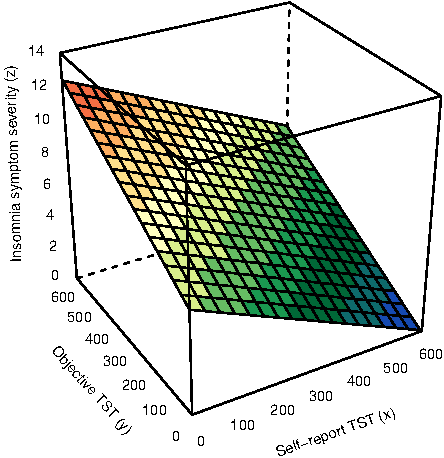
\includegraphics[width=0.4\linewidth]{methods_paper_files/figure-latex/diff-plot-1} }\subfloat[Additive model\label{fig:diff-plot-2}]{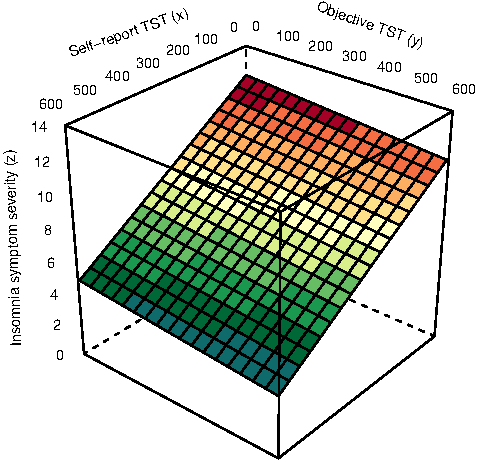
\includegraphics[width=0.4\linewidth]{methods_paper_files/figure-latex/diff-plot-2} }

}

\caption{Difference score and additive model plots}\label{fig:diff-plot}
\end{figure}

\noindent\emph{Note.} The equal but opposite respective effects of self-report TST and objective TST in insomnia symptom severity in the difference score model can be observed by inspecting the slopes directly above the x and y axes, respectively. By contrast, the slope above the y axis denoting values of objective TST in the additive model is very close to zero. In this latter case, the plot could be reduced to two dimensions without any loss of information, consistent with a unique effect of only one of two predictors.

As evident from the preceding demonstration, constraints imposed by the difference score were inappropriate and associated with a statistically significant decrement in prediction. Furthermore, the additive model, where coefficients for sTST and oTST were free to take on any value, revealed no unique contribution from oTST and that insomnia severity index scores were best predicted by sTST alone. In other words, holding sTST constant and increasing or decreasing objective sleep time will not correspond to a change in predicted insomnia symptom severity. This outcome is entirely inconsistent with any kind of discrepancy effect and it is possible that this could be reproduced in any sleep discrepancy study employing difference scores in the same way demonstrated.

\subsection{Absolute difference scores}\label{absolute-difference-scores}

\subsubsection{Directionality}\label{directionality-1}

The problem of directionality applies to absolute difference scores yet in a different way to their simple algebraic counterparts. Within a statistical relationship, absolute difference scores assume that the magnitude and direction of the effect will be symmetrical about a central value of 0. For sleep discrepancy, this means that negative discrepancy is assumed to be equivalent to positive discrepancy with respect to their relationship with another variable. This becomes an issue where the distribution of an analogous simple algebraic difference score does not meaningfully occupy both sides of zero. For example, in a sample where negligible sleep overestimation is present (unlike our example depicted in Figure \ref{fig:histogram}), a result indicating a significant relationship of absolute sleep agreement with another variable would be driven entirely by negative sleep discrepancy---an outcome very different to a naive interpretation of the results. In fact, any substantial skew in the distribution of an equivalent simple algebraic difference score about the 0-value would call into question the choice for absolute difference in this respect.

\subsubsection{Implicit weightings of difference score components}\label{implicit-weightings-of-difference-score-components}

Absolute difference scores impose implicit weightings on coefficients that represent the symmetry introduced in the previous paragraph, in addition to constraints analogous to that of simple algebraic difference scores. Edwards (2002) provides demonstrations in equation form by using a dummy variable (W) in a piecewise regression\footnote{Note. This dummy variable approach to piece-wise regression is distinct to the approach used to demonstrate directionality problems with difference scores. The dummy variable sets the breakpoint at sTST = oTST which optimally should be estimated empirically. Unfortunately, methods for estimating breakpoints empirically across two or more linear combinations of predictors do not appear to be presently available in R.}. In the case of insomnia and sleep discrepancy W is equal to 0 when e.g., \(sTST > oTST\), and 1 when \(sTST \le oTST\).

\begin{equation}
ISI = b_{0} + b_{1} (1 - 2W)(sTST - oTST) + \epsilon
\label{eq:absolute}
\end{equation}

For positive (and no) sleep discrepancy the term (1 - 2W) will equal 1 and for negative sleep discrepancy it will equal -1, effectively reversing the sign of \(sTST - oTST\). Equation \eqref{eq:absolute} can be expanded to provide

\begin{equation}
ISI = b_{0} + b_{1}sTST - b_{1}oTST - 2b_{1}W sTST + 2b_{1}W oTST + \epsilon
\label{eq:absolute2}
\end{equation}

The weightings applied to the coefficients in \eqref{eq:absolute2} can be made explicit with comparison to the following unconstrained piecewise linear equation containing sTST and oTST as separate predictors.

\begin{equation}
ISI = b_{0} + b_{1}sTST + b_{2}oTST + b_{3}W + b_{4}W sTST + b_{5}W oTST + \epsilon
\label{eq:absolute3}
\end{equation}

Comparing equations \eqref{eq:absolute2} and \eqref{eq:absolute3} reveals the following constraints \(b_{1} = - b_{2}\), \(b_{4} = - b_{5}\), \(b_{3} = 0\), and \(b_{4} = -2b_{1}\) (Edwards, 2002). This may be expressed more intuitively by separating equations according to the value of dummy variable W.

\begin{equation}
\begin{split}
ISI_{sTST \le oTST} & = b_{0} + b_{1}sTST + b_{1}oTST - 2b_{1}(1) sTST + 2b_{1}(1) oTST + \epsilon \\
& = b_{0} - (1)b_{1}sTST + b_{1}oTST + \epsilon
\end{split}
\label{eq:absolute4a}
\end{equation}

\begin{equation}
\begin{split}
ISI_{sTST > oTST} & = b_{0} + b_{1}sTST + b_{1}oTST - 2b_{1}(0) sTST + 2b_{1}(0) oTST + \epsilon \\
& = b_{0} + b_{1}sTST - (1)b_{1}oTST + \epsilon
\end{split}
\label{eq:absolute4b}
\end{equation}

Absolute difference scores thus weight the respective effects of sTST and oTST as equal in magnitude but opposite in sign, with each valence reversing at the sTST = oTST line, imposing a symmetry on predicted values of ISI. There is little reason, empirical or theoretical, to believe that the relationship of sleep time discrepancy to insomnia will be identical for negative versus positive discrepancy.

A further problem can be observed by considering the sTST = oTST line where self-report and objective estimates of TST are perfectly congruent. The slope and intercept of this line for the absolute difference score model and unconstrained piecewise model can be found by substituting sTST = oTST into equations \eqref{eq:absolute} and \eqref{eq:absolute3}. For the absolute difference model:

\begin{equation}
\begin{split}
ISI & = b_{0} + b_{1}sTST - b_{1}sTST - 2b_{1}W sTST + 2b_{1}W sTST + \epsilon \\
& = b_{0} + \epsilon
\end{split}
\label{eq:absolute5a}
\end{equation}

The sTST = oTST line consists of only an intercept and thus remains perfectly flat across the dimension represented by predicted values of ISI. This represents a further assumption that there is no combined main effect of sTST and oTST on ISI that would be represented by a slope in this line.

Compare with the unconstrained piecewise model:

\begin{equation}
\begin{split}
ISI & = b_{0} + b_{1}sTST + b_{2}sTST + b_{3}W + b_{4}W sTST + b_{5}W sTST + \epsilon \\
ISI_{sTST \le oTST} & = b_{0} + (b_{1} + b_{2})sTST + \epsilon
\end{split}
\label{eq:absolute5b}
\end{equation}

\begin{equation}
\begin{split}
ISI & = b_{0} + b_{1}sTST + b_{2}sTST + b_{3}W + b_{4}W sTST + b_{5}W sTST + \epsilon \\
ISI_{sTST > oTST} & = (b_{0} + b_{3}) + (b_{1} + b_{2} + b_{3} + b_{4})sTST + \epsilon
\end{split}
\label{eq:absolute5c}
\end{equation}

The second bracketed term in Equations \eqref{eq:absolute5b} and \eqref{eq:absolute5c} implies that there is a discontinuity in predicted values of ISI at the sTST = oTST line with each part of the function having an independent slope and intercept.

Empirical support for the coefficient weights described above can be illustrated using the same data as used in the example for difference scores. Equations \eqref{eq:absolute} and \eqref{eq:absolute3} can be estimated and coefficients observed in Table \ref{tab:absolutereg}.

\begin{table}[!h]
\centering
\caption{\label{tab:absolutereg}Absolute diffference score and unconstrained piecewise regression}
\centering
\fontsize{10}{12}\selectfont
\begin{threeparttable}
\begin{tabular}[t]{llllll}
\toprule
  & Estimate & 95\% CI [LL, UL] & Standard Error & t-value & p-value\\
\midrule
\addlinespace[0.3em]
\multicolumn{6}{l}{\textbf{Absolute difference model}}\\
\hspace{1em}Intercept & 6 & {}[5.62 , 6.38] & 0.194 & 30.9 & < .001\\
\addlinespace
\hspace{1em}absTST & 0.014 & {}[0.009 , 0.019] & 0.003 & 5.57 & < .001\\
\addlinespace
\addlinespace[0.3em]
\multicolumn{6}{l}{\textbf{Unconstrained piecewise model}}\\
\hspace{1em}Intercept & 8.98 & {}[6.06 , 11.9] & 1.49 & 6.02 & < .001\\
\addlinespace
\hspace{1em}sTST & 0.004 & {}[-0.009 , 0.017] & 0.007 & 0.612 & .541\\
\addlinespace
\hspace{1em}oTST & -0.012 & {}[-0.026 , 0.002] & 0.007 & -1.66 & .097\\
\addlinespace
\hspace{1em}W & 4.31 & {}[0.221 , 8.4] & 2.08 & 2.07 & .039\\
\addlinespace
\hspace{1em}W*sTST & -0.018 & {}[-0.032 , -0.004] & 0.007 & -2.48 & .013\\
\addlinespace
\hspace{1em}W*oTST & 0.01 & {}[-0.006 , 0.027] & 0.008 & 1.26 & .209\\
\addlinespace
\bottomrule
\end{tabular}
\begin{tablenotes}[para]
\item \textit{Note: } 
\item CI = confidence intervals, LL = lower limit, UL = upper limit, absTST = absolute difference score of sTST and oTST, W = dummy variable coding when $sTST \le oTST$, W*sTST and W*oTST are extra terms present in the model for when $sTST \le oTST$
\end{tablenotes}
\end{threeparttable}
\end{table}

The coefficient of determination from the unconstrained piecewise regression (R\textsuperscript{2} = .072) was increased more than two-fold from the absolute difference score model (R\textsuperscript{2} = .03), a difference that was statistically significant (\emph{F} = 11.2, \emph{p} = \textless{} .001). Hence, the coefficient weights imposed by the absolute difference model (see Figure \ref{fig:abs-plot}a) are not supported by the data when compared to the unconstrained piecewise model (see Figure \ref{fig:abs-plot}b). Furthermore, for the unconstrained piecewise model, greater insomnia symptom severity is associated with increased self-report sleep when sTST \textgreater{} oTST and decreased self-report sleep when sTST \textless{} oTST, with the latter effect somewhat stronger than the former, as indicated by a steeper slope. On the other hand, oTST appears to have a negligible effect. Therefore, as with the empirical demonstration for simple algebraic difference scores, there is no presence of a discrepancy effect.

\begin{figure}

{\centering \subfloat[Absolute difference score model\label{fig:abs-plot-1}]{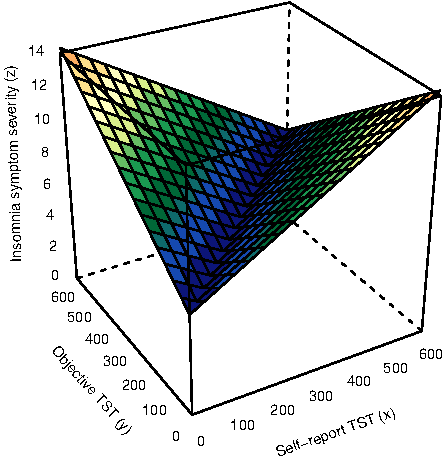
\includegraphics[width=0.4\linewidth]{methods_paper_files/figure-latex/abs-plot-1} }\subfloat[Unconstrained piecewise model\label{fig:abs-plot-2}]{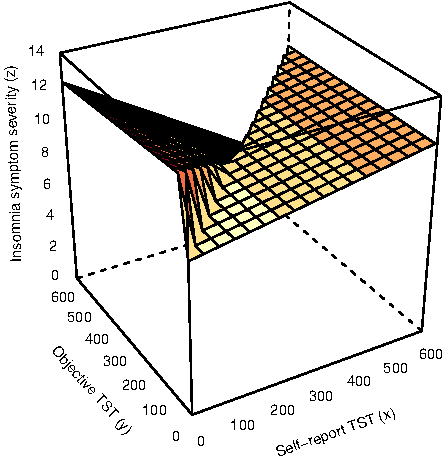
\includegraphics[width=0.4\linewidth]{methods_paper_files/figure-latex/abs-plot-2} }

}

\caption{Absolute difference score and unconstrained piecewise model plots}\label{fig:abs-plot}
\end{figure}

\noindent\emph{Note.} The constraints imposed by the absolute difference score model can be observed by inspecting the V-shaped surface in Figure \ref{fig:abs-plot}a that is symmetric about the X = Y line. This is in contrast to \ref{fig:abs-plot}b where a discontinuity is present at the x = y line and the slopes denoting the effects of self-report and objective sleep are free to take on different values.

The values of the constrained coefficients in the absolute difference score model can be estimated, as in the demonstration of algebraic difference scores. This expanded absolute difference score model is available in Table \ref{tab:absoluteexpanded}.

\begin{table}[!h]
\centering
\caption{\label{tab:absoluteexpanded}Expanded absolute difference score model}
\centering
\fontsize{10}{12}\selectfont
\begin{threeparttable}
\begin{tabular}[t]{llllll}
\toprule
  & Estimate & 95\% CI [LL, UL] & Standard Error & t-value & p-value\\
\midrule
Intercept & 6 & {}[5.7 , 6.31] & 0.191 & 5.61 & 6.36\\
sTST & 0.014 & {}[0.01 , 0.018] & 0.003 & 0.009 & .019\\
oTST & -0.014 & {}[-0.018 , -0.01] & 0.003 & -0.019 & < .001\\
W & 0 &  &  &  & \\
W*sTST & -0.028 & {}[-0.036 , -0.019] & 0.005 & -0.038 & < .001\\
\addlinespace
W*oTST & 0.028 & {}[0.019 , 0.036] & 0.005 & 0.017 & .038\\
\bottomrule
\end{tabular}
\begin{tablenotes}[para]
\item \textit{Note: } 
\item CI = confidence intervals, LL = lower limit, UL = upper limit, absTST = absolute difference score of sTST and oTST, W = dummy variable coding when $sTST \le oTST$, W*sTST and W*oTST are extra terms present in the model for when $sTST \le oTST$. Confidence intervals were derived from 1000 bootstrapped samples.
\end{tablenotes}
\end{threeparttable}
\end{table}

\subsection{Ratio scores}\label{ratio-scores}

\subsubsection{Directionality}\label{directionality-2}

Ratio scores, similar to difference scores, operationalise sleep discrepancy as a spectrum in one-dimensional space (see Table \ref{tab:samples}). Unlike difference scores however, ratio score values are all positive, with negative or positive sleep discrepancy represented either side of a central value of 1. As such, the directionality problem exists for ratio scores as it does for algebraic difference scores.

\subsubsection{Implicit weighting of ratio score components}\label{implicit-weighting-of-ratio-score-components}

Ratio scores impose weightings or constraints on regression coefficients, although in a manner that is more difficult to express than for difference scores. The effects of the components of a ratio score within a regression can be provided by partial derivatives (Stolzenberg, 2021).

Using the example of the regression of ISI on sTST/oTST (or rTST), the partial derivative of ISI with respect to sTST (and thus the effect of sTST on predicted values of ISI) is provided by:

\begin{equation}
\begin{split}
\frac{\partial{\hat{ISI}}}{\partial{sTST}} & = [\frac{\partial}{\partial{sTST}}b_{1}{sTST}][\frac{1}{oTST}] \\
& = \frac{b_{1}}{oTST}
\end{split}
\label{eq:partial1}
\end{equation}

Whilst the partial derivative of ISI with respect to oTST to is:

\begin{equation}
\begin{split}
\frac{\partial{\hat{ISI}}}{\partial{sTST}} & = [\frac{\partial}{\partial{oTST}} b_{1}{oTST}^{-1}][{sTST}] \\
& = [-b_{1}{oTST}^{-2}][{sTST}] \\
& = \frac{-b_{1}{sTST}}{{oTST}^{2}}
\end{split}
\label{eq:partial2}
\end{equation}

Multiplying the Equations \eqref{eq:partial1} and \eqref{eq:partial2} by \(oTST^{2}\) provides \(b_{1}oTST\) and \(-b_{1}sTST\), respectively. Hence, the respective contributions of each ratio score component are opposite in sign and vary as a function of the other component. This is similar to the coefficient weightings imposed by difference scores, albeit with a non-linearity introduced into the implied functional form. Recall the change in differences between row values in Table \ref{tab:samples} for the sample ratio scores provided. The results of this are akin to a data transformation and can be visualised, as in previous examples, by plotting regressions with components considered as separate predictors. See Figure \ref{fig:ratio-plot}.

\begin{figure}
\centering
\pandocbounded{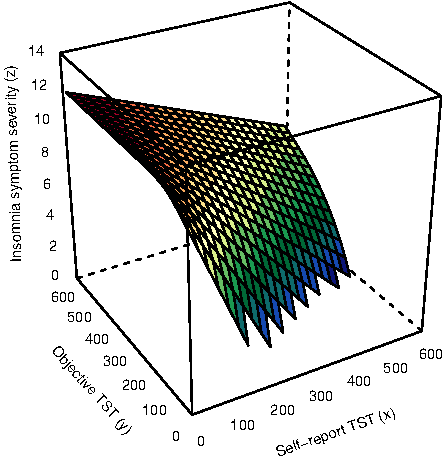
\includegraphics[keepaspectratio]{methods_paper_files/figure-latex/ratio-plot-1.pdf}}
\caption{\label{fig:ratio-plot}Ratio regression plot}
\end{figure}

\noindent\emph{Note.} In the ratio regression plot we can observe insomnia severity is maximised where objective sleep most exceeds self-report sleep, with a sharp non-linear decline across the y axis until the figure moves beyond the boundary of positive z values.

The non-linear functional form implied by a ratio score regression may reflect a discrepancy effect (as seen in Figure \ref{fig:ratio-plot}, but the coefficient weightings are unlikely to be supported empirically and are very difficult to interpret or define a priori (i.e., for a hypothesis).

An alternative example can be provided by expressing the ratio in exponential terms:

\begin{equation}
ISI = b_{0}+b_{1}sTST \cdot oTST^{-1} + \epsilon
\label{eq:lmrat2}
\end{equation}

Here, the regression can be seen as a test of the interaction between sTST and the reciprocal of oTST but with first-order terms missing for each predictor (Bradshaw \& Radbill, 1987). As a result, the interaction term will combine explained variance from both sTST and \(oTST^{-1}\) (Wiseman, 2009). This is a form of constraint that can be relaxed by adding the first-order terms for each component:

\begin{equation}
= b_{0} + b_{1}sTST + b_{2}oTST^{-1} + b_{3}(sTST \cdot oTST^{-1}) + \epsilon
\label{eq:lmrat3}
\end{equation}

Past authors have recommended that ratio scores be used only when their components are included as first-order terms (Kronmal, 1993). Unfortunately, the test of an interaction is only a test of discrepancy when the two predictors are categorical (e.g., within ANOVA), rather than continuous, making this method inappropriate for operationalising discrepancy in sleep time parameters. See Edwards (2001) for further discussion of this particular problem.

Constraints implicit in the ratio regression can be tested empirically in the same manner as in previous examples. The ratio score model and the unconstrained interaction model \eqref{eq:lmrat3} are estimated with coefficients available in Table \ref{tab:ratio-tests}.

\begin{table}[!h]
\centering
\caption{\label{tab:ratio-tests}Ratio score model and unconstrained interaction with inverse oTST model}
\centering
\fontsize{10}{12}\selectfont
\begin{threeparttable}
\begin{tabular}[t]{llllll}
\toprule
  & Estimate & 95\% CI [LL, UL] & Standard Error & t-value & p-value\\
\midrule
\addlinespace[0.3em]
\multicolumn{6}{l}{\textbf{Ratio score model}}\\
\hspace{1em}Intercept & 11.9 & {}[10.3 , 13.6] & 0.843 & 14.2 & < .001\\
\hspace{1em}rTST & -5.42 & {}[-7.08 , -3.76] & 0.847 & -6.4 & < .001\\
\addlinespace[0.3em]
\multicolumn{6}{l}{\textbf{Unconstrained interaction model}}\\
\hspace{1em}Intercept & 8.16 & {}[1.71 , 14.6] & 3.29 & 2.48 & .013\\
\hspace{1em}sTST & -0.009 & {}[-0.016 , -0.003] & 0.004 & -2.7 & .007\\
\hspace{1em}oTST\textasciicircum{}-1 & 401 & {}[-585 , 1387] & 502 & 0.798 & .425\\
sTST*oTST\textasciicircum{}-1 & 1.27 & {}[-0.519 , 3.07] & 0.914 & 1.39 & .164\\
\bottomrule
\end{tabular}
\begin{tablenotes}[para]
\item \textit{Note: } 
\item CI = confidence intervals, LL = lower limit, UL = upper limit, rTST = ratio score of sTST/oTST, sTST*oTST\textasciicircum{}-1 = interaction (product) term of sTST and the inverse of oTST, sTST = self-report total sleep time, oTST = objective total sleep time
\end{tablenotes}
\end{threeparttable}
\end{table}

A statistically significant increase in R\textsuperscript{2} from the the ratio score model (R\textsuperscript{2} = .023) to the unconstrained (R\textsuperscript{2} = .059) model is observed (\emph{F} = 53.7, \emph{p} \textless{} .001), indicating a lack of empirical support for the constraints imposed by ratio scores. The unconstrained interaction model with inverse oTST is depicted in Figure \ref{fig:ratio-unc}.

\begin{figure}
\centering
\pandocbounded{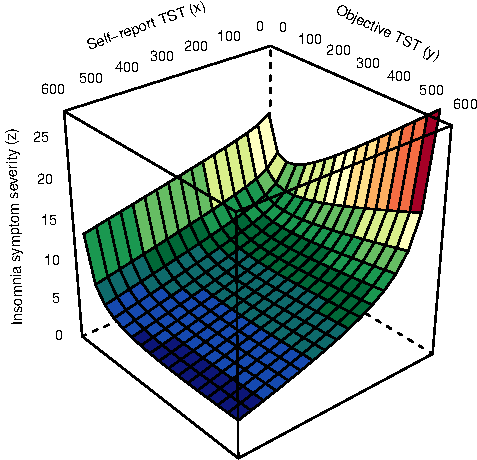
\includegraphics[keepaspectratio]{methods_paper_files/figure-latex/ratio-unc-1.pdf}}
\caption{\label{fig:ratio-unc}Unconstrained interaction model with inverse oTST}
\end{figure}

\noindent\emph{Note.} The product term and reciprocal transformation of oTST afford a bend in the surface representing predicted values of ISI. In this case, the model implies that insomnia symptom severity is minimised at higher values of both objective and self-report TST, increasing non-linearly at extreme low values of self-report TST and low values of objective TST. A principled approach to modelling discrepancy effects using complex surfaces resembling this one will be discussed in the section for response surface analysis.

\subsection{Derived indices as dependent variables}\label{derived-indices-as-dependent-variables}

In the preceding paragraphs, problems with derived indices have been discussed in the context of their use as independent variables. There are no substantive differences between using derived indices as predictors or outcomes when all variables are continuous. Continuing with the difference score dTST as an example, exchanging their previously defined places to predict dTST from ISI provides (Edwards, 1995):

\begin{equation}
\begin{split}
sTST-oTST & = b_{0}+b_{1}ISI + \epsilon \\
(1)sTST + (-1)oTST & = b_{0}+b_{1}ISI + \epsilon
\end{split}
\label{eq:lmdep}
\end{equation}

Predicted values of sTST and oTST are thus constrained to be equal in magnitude but opposite in sign with respect to the effect of the independent variable, ISI. Explicit demonstration of this is difficult as respective effects on the components of the dependent variable cannot be easily decomposed. However, with this simple bivariate regression, the proportion of variance accounted for by the model will be identical regardless of the designation of dTST as dependent or independent variable.

The case for discrepancy as a dependent variable is different with categorical independent variables, for instance, with the testing of differences between derived score means with t-tests or ANOVA. It makes less sense to speak of constraints here, as a derived index will either be lower or higher for each level of an independent variable. However, the directionality problem applies, and, in isolation, derived indices provide no information about the levels of their components. For example, a decreased difference score mean from time 1 to time 2 in a treatment study of Cognitive Behavioural Therapy for Insomnia (CBT-I) could reflect an increased self-report TST becoming more congruent with an unchanged objective TST as much as a decreased objective TST becoming more congruent with an unchanged self-report TST. Each case would lead to very different interpretations of a study. Whilst the latter situation is unlikely, there is no way to determine with certainty without also exploring the component (i.e., self-report TST, objective TST) means.

\section{Summary of problems}\label{summary-of-problems}

All the problems described above originate with the fundamental issue that a single derived index calculated from two component variables cannot provide any more information than its components considered separately. When included in regression-based procedures, a derived index imposes assumptions about the form of the relationship between its components and the outcome variable. Calculating derived indices involves a necessary loss of information unless, by chance, the constrained relationship implied by the derived index is exactly supported by the data. Edwards (2002) describes this problem as one of dimensional reduction---the collapse of a 3-dimensional relationship between three separate variables to an equivocal two-dimensional one. The empirical demonstrations in the preceding paragraphs reveal that the assumptions implicit in the use of derived indices are not borne out by sleep data and that the use of these scores is inadequate to characterise more complex underlying relationships.

More broadly, sleep discrepancy, defined as the discordance between self-report and objective sleep, is a deceptively complex concept to operationalise. In fact, the terms discrepancy, congruence, discordance etc\ldots{} do little to describe an actual statistical relationship in mathematical terms and a verbal hypothesis where they are included is at substantial risk of being completely underspecified. As such, the use of derived indices should not be considered merely a small methodological issue that could affect some results, but a fundamental failure to test the hypotheses necessary to build theory in this area.

\section{Solutions}\label{solutions}

There is a range of approaches that aim to mitigate or resolve the problems with derived indices discussed in the above paragraphs. These strategies are introduced briefly below with a discussion for their appropriateness for the investigation of sleep discrepancy.

\subsection{A note about directed versus non-directed difference}\label{a-note-about-directed-versus-non-directed-difference}

In all discussions provided above, self-report and objective TST and the insomnia severity index (ISI) were used as examples. There may be cases for which an outcome is expected to be related linearly across all levels of a self-report and objective sleep variable. For example, sleep onset latency (SOL), by some objective definitions, is rarely underestimated (Saline et al., 2016; \textbf{hermans2020onset?}) and sleep discrepancy on this metric could be expected to correspond to increasing insomnia symptom severity linearly throughout its entire observed range. This directional form of discrepancy has been referred to as ``directed difference'' to contrast with the more complex discrepancy i.e., ``non-directed difference'' that may see an effect change throughout the range of self-report or objective sleep Schönbrodt (2016). Accordingly, the directionality problem explained in the preceding sections is a result of applying a directed difference approach where non-directed difference would be more appropriate.

\subsection{Categorising difference scores}\label{categorising-difference-scores}

Categorising difference scores into groups based on their values is a common strategy in the sleep discrepancy literature (Walton et al., 2025). For example, participants may be assigned membership to an ``underestimator'' category if their dTST is below 50, an ``overestimator'' category if their dTST is over 50, and a ``normal estimator'' category if their dTST is between the prior two values, with an ANOVA conducted to test differences in means for some outcome. This strategy can address issues with directionality when enough categories are specified (\textbf{aiken1991?}). Unfortunately, however, categorising continuous measures results in a reduction in statistical power that can be substantial (Edwards, 2001). An additional problem is introduced by the decision of where to place the cut-points for group membership, which, without support of theory or the data itself, is arbitrary.

\subsection{Subgroup analyses}\label{subgroup-analyses}

Another potential solution to the directionality problem is to run separate analyses for negative and positive sleep discrepancy. However, if separate analyses are conducted on difference scores (e.g., either side of dTST = 0), problems of implicit coefficient weights remain and statistical power is reduced through the splitting of the sample. The decision of where to split the sample, too, remains arbitrary, and ideally should be tested for empirically.

\subsection{The additive model and condition-based regression analysis}\label{the-additive-model-and-condition-based-regression-analysis}

The additive model, composed of a regression with sTST and oTST as separate linear predictors, was demonstrated in a previous example and provided more information than the accompanying difference score regression. If a researcher is interested in measuring a relationship of discrepancy to an outcome that is linear across all levels of self-report and objective sleep (i.e., a directed difference) then this approach may be useful. Support for a discrepancy hypothesis could be provided by observing statistically significant unique contributions of each sleep measure that are opposite in sign. As a test of directed difference, however, this approach would not be appropriate for a hypothesis where the effect of discrepancy changes at any value of the predictors. Humberg et al. (2018) devised a formal method for assessing coefficients in the additive model for adherence to the coefficient pattern consistent with directed discrepancy described above. This procedure, called condition-based regression analysis, is intuitively described and has the advantage of combining coefficient tests into a single hypothesis test.

\subsection{Latent difference score modelling}\label{latent-difference-score-modelling}

Alternatives for investigating directed difference are approaches based in structural equation modelling (SEM) such as Cheung (2009)'s Latent Congruence Model or the procedure described by McArdle (2009). These techniques involve using higher order latent factors with specified factor loadings to represent the differences between components of a derived score. This addresses the problem of implicit constraints associated with difference scores, allowing for coefficients to be empirically weighted in the model. Advantages of SEM-based approaches include the ability to account for measurement error, assess for measurement invariance, and the considerable flexibility in model specification. The first two advantages may not be as applicable for sleep time discrepancy as in, for example, individual differences research, but the flexibility of SEM could prove extremely useful for theory building in this area. For example, latent difference scores can be specified as antecedents or consequents in relation to any number of latent or observed variables. For the present, latent difference score modelling is unable to represent complex relationships necessary for testing non-directed difference.

\subsection{Spline regression}\label{spline-regression}

Spline regression, introduced to discrepancy by Edwards \& Parry (2018), is an approach to investigating non-directed difference that overcomes problems associated with the use of of absolute difference scores. Similar to the piecewise approach demonstrated in a previous section, empirically-estimated points that allow changes in slopes provide the complexity required to represent a discrepancy effect. Spline regression treats the components of an absolute difference score as separate predictors of an outcome, expanding the model to three dimensions. Therefore, rather than breakpoints, spline regression estimates \emph{seams} along a regression surface where slopes may change. The general equation for a spline regression with a single seam is (Edwards \& Parry, 2018):

\begin{equation}
Z = b_{0} + b_{1}X + b_{2}Y + b_{3}(Y - c_{0} - c_{1}X)(Y < c_{0} + c_{1}X) + \epsilon
\label{eq:spline}
\end{equation}

where \(Y < c_{0} + c_{1}X\) is a logical expression allowing the slopes of the surface to change depending on the region demarcated by the seam defined by \(Y = c_{0} + c_{1}X\). Support for a non-directed discrepancy hypothesis is provided by a seam that lies along the X = Y line, corresponding to exactly equal predictor combinations.

As a less constrained form of the absolute difference score model, spline regression can test the constraints on coefficient weights imposed by these difference scores empirically and allow for surfaces that are asymmetrical (i.e., having differing slopes) about the seam. Adding to this flexibility is the potential for estimating multiple seams from which flat zones can be estimated where the predicted values of the outcome remain constant.

To date, there appears to be no use of this procedure outside of the demonstration provided by Edwards \& Parry (2018) in the paper where it was introduced. A formal approach to hypothesis testing is yet to be developed. Edwards \& Parry (2018) estimate parameters with nonlinear regression and as models are nested, R\textsuperscript{2} can be used for model comparison. Bootstrapped confidence intervals may be used to investigate the offset and rotation of a seam on the X = Y line or any other region of theoretical interest.

\subsection{Polynomial regression with response surface analysis}\label{polynomial-regression-with-response-surface-analysis}

Polynomial regression with response surface analysis (Edwards, 2002; Humberg et al., 2019) is an approach that allows for the testing of non-directed difference that overcomes problems with derived indices described in the preceding sections. In this approach, components of a derived index are entered as separate predictors in a polynomial model with their squared terms and an interaction.

\begin{equation}
Z = b_{0} + b_{1}X + b_{2}Y + b_{3}X^{2} + b_{4}XY + b_{5}Y^{2}
\label{eq:rsa}
\end{equation}

Predicted values of Z form a complex shape in 3-dimensional space (i.e., a response surface) that can be tested at various key points to test support for a discrepancy effect. Where spline regression uses estimated breakpoints or seams to provide the complexity required for testing discrepancy, response surface analysis uses higher order terms. As such, the latter approach makes an assumption of differentiability or ``smoothness'' about the point where an outcome is maximised or minimised. The polynomial model in equation \eqref{eq:rsa} can be seen as a less constrained version of that implied by the squared difference score--a derived index absent in the sleep discrepancy literature but used elsewhere in a similar manner to an absolute difference.

\begin{equation}
Z = b_{0} + b_{1}(X - Y)^{2}
\label{eq:squareddifference}
\end{equation}

Expands to

\begin{equation}
Z = b_{0} + b_{1}X^{2} + - 2b_{1}XY - b_{1}Y^{2}
\label{eq:expanded}
\end{equation}

Equation \eqref{eq:squareddifference} is thus identical to Equation \eqref{eq:rsa} with the constraints that \(b_{1}\) and \(b_{2}\) = 0, \(b_{3}\) = \(b_{5}\), and \(-b_{4}\) = \(-2b_{3}\) (Edwards, 2002). The inclusion of \(b_{1}\) and \(b_{2}\) frees constraints and allows the testing of the main effects of the components of discrepancy in addition to the effect of discrepancy between the two predictors. See Edwards (2002) and Humberg et al. (2019) for detailed descriptions of response surface analysis.

Response surface analysis is traditionally performed by first estimating a polynomial regression and then testing the resulting surface for adherence to a discrepancy hypothesis (Edwards, 2002). An alternative approach involves comparing models with varying constraints within a model-testing framework, which can preserve statistical power (Schönbrodt, 2016). Complex discrepancy hypotheses including asymmetric (differing relationship when X \textgreater{} Y than when X \textless{} Y) and level-dependent (strength of discrepancy effect depends on the levels of the predictors) models can be tested by adding third-order terms to Equation \eqref{eq:rsa} and following the procedure introduced by Humberg et al. (2022). Whilst response surface analysis is more complex than regression-based analyses, the process and its graphical results are visually intuitive and software is available in R (Schönbrodt \& Humberg, 2023).

\subsection{Alternative study designs}\label{alternative-study-designs}

Defining relationships of discrepancy in sleep time parameters with other variables is a complex process that requires sophisticated statistical alternatives to avoid the problems associated with derived indices. Fortunately, this is not the only way to operationalise sleep discrepancy. For instance, experimental awakening paradigms allow participants to be queried about their sleep state when asleep or awake in the laboratory. A study structured in this way operationalises sleep discrepancy as a binary variable or confusion matrix that can be incorporated into any traditional approach to statistical inference. Repeated awakenings for a single participant is also beneficial for maximising power. Theoretically, the form of sleep discrepancy measured by these procedures is closer to the concept of direct discordance in sleep/wake states (Walton et al., 2025), which may be preferable to that defined by sleep time parameters, depending on the aims of the study. Alternative metrics for operationalising sleep discrepancy can capture the concept of discrepancy within their definition in a way that is not possible with derived indices. For example, Saline et al. (2016) measured the amount of objective sleep during the period defined by their participants' self-reported sleep latency in a series of polysomnography recordings. This index, known as sleep during subjective sleep latency (SDSL), does not involve any mathematical functions in its derivation and is not affected by the problems inherent to difference or ratio scores. Another alternative operationalisation makes use of mathematical modelling. (\textbf{hermans2020modelling?}) used sleep bout length \(L_s\) as a modelled parameter to minimise the root mean square error (RMSE) in prediction of self-reported sleep latency. Hence, \(L_s\) serves as a best estimate for the minimum bout length of sleep to be perceived as sleep and can be used to compare sleep misperception between groups.

\subsection{Conclusion}\label{conclusion-1}

There are significant conceptual and methodological problems associated with the use of derived indices including difference, ratio, and combination scores, in sleep discrepancy research. Sophisticated statistical alternatives are needed to define relationships of sleep time parameters with other outcomes. For simple discrepancy hypotheses, where the effects of the predictors are not expected to change throughout their range (i.e., directed difference), Humberg et al. (2018)'s condition-based regression or latent difference score modelling should be used. For more complex discrepancy hypotheses, where the effect of discrepancy is represented by the minimisation or maximisation of an outcome across a region defined by the predictors (i.e., non-directed difference), spline regression or response surface analysis should be used. See Figure \ref{fig:flowcharta} for an algorithmic depiction of derived index alternatives. For all studies investigating discrepancy, verbal hypotheses should specify the nature of the expected relationship as the term ``discrepancy'' does not, in itself, represent sufficient information to make meaningful testable predictions. Adoption of the alternatives described will not only vastly improve methodology in sleep discrepancy but allow stronger scientific inferences to be made. Indeed, hypothesised discrepancy effects, as specific functional forms describing complex relationships between three or more variables, are more precise than directional hypotheses (e.g., when x is higher, y will be higher) common to cross-sectional research. Consequently, they represent ``riskier predictions'' (\textbf{meehl1992?}), entailing phenomena that, absent a theory in question, would seem unlikely---or as (\textbf{salmon1984?}) calls ``an improbable coincidence''. More recently, these ideas have been reformulated by Mayo \& Spanos (2006) who has emphasised the \emph{severity} of a test as fundamental to valid inference, and a principle that transcends scientific-philosophical orientations.

\begin{figure}
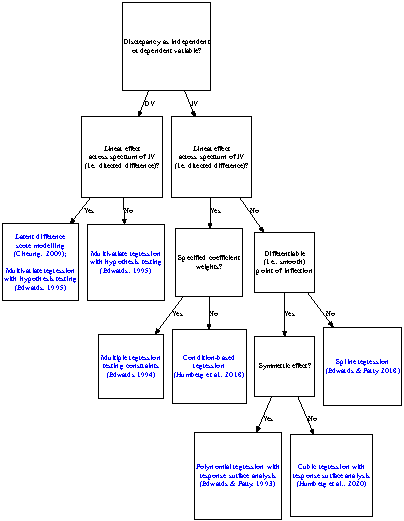
\includegraphics[width=1\linewidth]{methods_paper_files/figure-latex/flowcharta-1} \caption{Analytic strategies for investigating congruence and discrepancy}\label{fig:flowcharta}
\end{figure}

\noindent\emph{Note.} DV = dependent variable, IV = independent variable.

\section{Appendix}\label{appendix}

\subsection{Reduced reliabilities}\label{reduced-reliabilities}

Reliability problems are perhaps the best known issue with difference scores and are also present with ratio scores. Reliability has not been discussed in the main text as we perceive this problem to be less important than the others described above, particularly for sleep discrepancy research. A discussion of the reliability of derived indices is included below for the sake of completeness.

Where there is correlation between the components of a difference or ratio score, the reliability of that score will necessarily be lower than the average of the reliabilities of the components. This can be observed through the equation of the reliability of a difference score (Stanley, 1967) depicted below. Here, \sigma is the standard deviation, \(r_{xx}\) the reliability of x, and \(r_{xy}\) the correlation between x and y.

\begin{equation}
r_{(x-y)} = \frac{σ_{x}^{2}r_{xx}+σ^{2}_{y}r_{xy}-2r_{xy}σ_{x}σ_{y}}{σ^{2}_{x}+σ^{2}_{y}-2r_{xy}σ_{x}σ_{y}}
\label{eq:rxx1}
\end{equation}

Note that the reliability of x-y will only equal the average of its components when the term \(-2r_{xy}σ_{x}σ_{y}\), containing the correlation of x and y is set to zero. This point can be further illustrated with the example difference score dTST, composed in this case, of the subtraction of polysomnography (PSG) defined objective TST from a diary measure of self-report TST. The formula above can be plot as a function of the correlation \(r_{xy}\) and the average reliabilities of sTST and oTST (see Figure \ref{fig:reliability}).

\begin{figure}
\centering
\pandocbounded{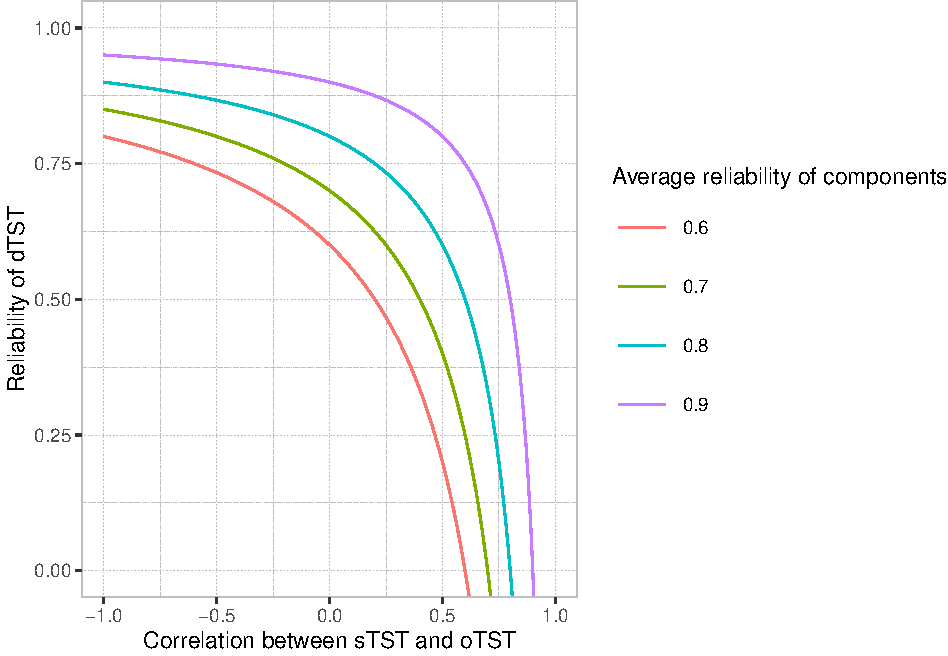
\includegraphics[keepaspectratio]{methods_paper_files/figure-latex/reliability-1.pdf}}
\caption{\label{fig:reliability}Reliability of dTST as a function of the correlation of its components}
\end{figure}

As the correlation between sTST and oTST approaches the average reliability of the two variables, the reliability of the difference score, dTST, approaches zero. A reliability of dTST equal or greater to the average of its components can be observed only when the correlation between sTST and oTST is zero or negative---each an unlikely case. Sleep measures are difficult to assess along traditional psychometric lines. For objective sleep, one study estimated the inter-rater reliability of scored sleep versus wake for PSG at .7 (Lee et al., 2022). On the self-report side, psychometric evaluations of sleep diary responses, for example, are not readily available. Night to night variability in sleep makes test-retest reliability difficult to assess and the different constructs tapped by each item render internal consistency reliability inappropriate (Carney et al., 2012; \textbf{dietch2021?}). Psychometric evaluations of self-report sleep time measures may be a fruitful area for further study.

Returning to derived indices, reduced reliabilities can be equally observed for ratio scores. The formula for the reliability of a ratio score \(r_{\frac{x}{y}}\) where \emph{cv} is equal to the coefficient of variation, \({\frac{\sigma}{M}}\) (Cronbach, 1941) is depicted below.

\begin{equation}
r_{\frac{x}{y}} = \frac{cv_{x}^{2}r_{xx}+cv^{2}_{y}r_{xy}-2r_{xy}cv_{x}cv_{y}}{cv^{2}_{x}+cv^{2}_{y}-2r_{xy}cv_{x}cv_{y}}
\label{eq:rxx2}
\end{equation}

The only substantive differences between these two cases is the replacement of the standard deviation \(σ\) with the coefficient of variation \(cv\) in the latter instance.

\phantomsection\label{refs}
\begin{CSLReferences}{1}{0}
\bibitem[\citeproctext]{ref-rmarkdown}
Allaire, J., Xie, Y., Dervieux, C., McPherson, J., Luraschi, J., Ushey, K., Atkins, A., Wickham, H., Cheng, J., Chang, W., \& Iannone, R. (2023). \emph{Rmarkdown: Dynamic documents for r}. \url{https://github.com/rstudio/rmarkdown}

\bibitem[\citeproctext]{ref-ancoli2015}
Ancoli-Israel, S., Martin, J. L., Blackwell, T., Buenaver, L., Liu, L., Meltzer, L. J., Sadeh, A., Spira, A. P., \& Taylor, D. J. (2015). The SBSM guide to actigraphy monitoring: Clinical and research applications. \emph{Behavioral Sleep Medicine}, \emph{13}(sup1), S4--S38.

\bibitem[\citeproctext]{ref-bradshaw1987}
Bradshaw, Y., \& Radbill, L. (1987). {Method and Substance in the Use of Ratio Variables}. \emph{American Sociological Review}, \emph{52}(1), 132. \url{https://doi.org/10.2307/2095398}

\bibitem[\citeproctext]{ref-carney2012}
Carney, C. E., Buysse, D. J., Ancoli-Israel, S., Edinger, J. D., Krystal, A. D., Lichstein, K. L., \& Morin, C. M. (2012). The consensus sleep diary: Standardizing prospective sleep self-monitoring. \emph{Sleep}, \emph{35}(2), 287--302.

\bibitem[\citeproctext]{ref-cheung2009}
Cheung, G. W. (2009). Introducing the {Latent} {Congruence} {Model} for {Improving} the {Assessment} of {Similarity}, {Agreement}, and {Fit} in {Organizational} {Research}. \emph{Organizational Research Methods}, \emph{12}(1), 6--33. \url{https://doi.org/10.1177/1094428107308914}

\bibitem[\citeproctext]{ref-cronbach1941}
Cronbach, L. J. (1941). The reliability of ratio scores. \emph{Educational and Psychological Measurement}, \emph{1}(1), 269--277.

\bibitem[\citeproctext]{ref-cronbach1970}
Cronbach, L. J., \& Furby, L. (1970). {How we should measure "change": Or should we?} \emph{Psychological Bulletin}, \emph{74}(1), 68--80. \url{https://doi.org/10.1037/h0029382}

\bibitem[\citeproctext]{ref-edinger1995}
Edinger, J. D., \& Fins, A. I. (1995). {The Distribution and Clinical Significance of Sleep Time Misperceptions Among Insomniacs}. \emph{Sleep}, \emph{18}(4), 232--239. \url{https://doi.org/10.1093/sleep/18.4.232}

\bibitem[\citeproctext]{ref-edwards1994}
Edwards, J. R. (1994). {The Study of Congruence in Organizational Behavior Research: Critique and a Proposed Alternative}. \emph{Organizational Behavior and Human Decision Processes}, \emph{58}(1), 51--100. \url{https://doi.org/10.1006/obhd.1994.1029}

\bibitem[\citeproctext]{ref-edwards1995}
Edwards, J. R. (1995). Alternatives to {Difference} {Scores} as {Dependent} {Variables} in the {Study} of {Congruence} in {Organizational} {Research}. \emph{Organizational Behavior and Human Decision Processes}, \emph{64}(3), 307--324. \url{https://doi.org/10.1006/obhd.1995.1108}

\bibitem[\citeproctext]{ref-edwards2001}
Edwards, J. R. (2001). Ten {Difference} {Score} {Myths}. \emph{Organizational Research Methods}, \emph{4}(3), 265--287. \url{https://doi.org/10.1177/109442810143005}

\bibitem[\citeproctext]{ref-edwards2002}
Edwards, J. R. (2002). {Alternatives to difference scores: Polynomial regression analysis and response surface methodology}. In F. Drasgow \& N. Schmitt (Eds.), \emph{Measuring and analyzing behavior in organizations: Advances in measurement and data analysis} (pp. 350--400). Jossey-Bass. \url{https://doi.org/10.1037/e576892011-020}

\bibitem[\citeproctext]{ref-edwards2018}
Edwards, J. R., \& Parry, M. E. (2018). On the {Use} of {Spline} {Regression} in the {Study} of {Congruence} in {Organizational} {Research}. \emph{Organizational Research Methods}, \emph{21}(1), 68--110. \url{https://doi.org/10.1177/1094428117715067}

\bibitem[\citeproctext]{ref-griffin1999}
Griffin, D., Murray, S., \& Gonzalez, R. (1999). {Difference score correlations in relationship research: A conceptual primer}. In \emph{Personal Relationships} (4; Vol. 6, pp. 505--518). \url{https://doi.org/10.1111/j.1475-6811.1999.tb00206.x}

\bibitem[\citeproctext]{ref-humberg2018}
Humberg, S., Dufner, M., Schönbrodt, F. D., Geukes, K., Hutteman, R., Van Zalk, M. H. W., Denissen, J. J. A., Nestler, S., \& Back, M. D. (2018). Enhanced versus simply positive: {A} new condition-based regression analysis to disentangle effects of self-enhancement from effects of positivity of self-view. \emph{Journal of Personality and Social Psychology}, \emph{114}(2), 303--322. \url{https://doi.org/10.1037/pspp0000134}

\bibitem[\citeproctext]{ref-humberg2019}
Humberg, S., Nestler, S., \& Back, M. D. (2019). Response {Surface} {Analysis} in {Personality} and {Social} {Psychology}: {Checklist} and {Clarifications} for the {Case} of {Congruence} {Hypotheses}. \emph{Social Psychological and Personality Science}, \emph{10}(3), 409--419. \url{https://doi.org/10.1177/1948550618757600}

\bibitem[\citeproctext]{ref-humberg2022}
Humberg, S., Schönbrodt, F. D., Back, M. D., \& Nestler, S. (2022). Cubic response surface analysis: {Investigating} asymmetric and level-dependent congruence effects with third-order polynomial models. \emph{Psychological Methods}, \emph{27}(4), 622--649. \url{https://doi.org/10.1037/met0000352}

\bibitem[\citeproctext]{ref-diagrammer}
Iannone, R. (2023). \emph{DiagrammeR: Graph/network visualization}. \url{https://CRAN.R-project.org/package=DiagrammeR}

\bibitem[\citeproctext]{ref-kronmal1993}
Kronmal, R. A. (1993). {Spurious Correlation and the Fallacy of the Ratio Standard Revisited}. \emph{Journal of the Royal Statistical Society: Series A (Statistics in Society)}, \emph{156}(3), 379--392.

\bibitem[\citeproctext]{ref-lee2022}
Lee, Y. J., Lee, J. Y., Cho, J. H., \& Choi, J. H. (2022). Interrater reliability of sleep stage scoring: A meta-analysis. \emph{Journal of Clinical Sleep Medicine}, \emph{18}(1), 193--202.

\bibitem[\citeproctext]{ref-lindsay2023}
Lindsay, D. S. (2023). A plea to psychology professional societies that publish journals: Assess computational reproducibility. \emph{Meta-Psychology}, \emph{7}.

\bibitem[\citeproctext]{ref-lubas2022}
Lubas, M. M., Szklo-Coxe, M., Mandrell, B. N., Howell, C. R., Ness, K. K., Srivastava, D. K., Hudson, M. M., Robison, L. L., Krull, K. R., \& Brinkman, T. M. (2022). Concordance between self-reported sleep and actigraphy-assessed sleep in adult survivors of childhood cancer: The impact of psychological and neurocognitive late effects. \emph{Support Care Cancer}, \emph{30}(2), 1159--1168. \url{https://doi.org/10.1007/s00520-021-06498-x}

\bibitem[\citeproctext]{ref-manconi2010}
Manconi, M., Ferri, R., Sagrada, C., Punjabi Naresh, M., Tettamanzi, E., Zucconi, M., Oldani, A., Castronovo, V., \& Ferini-Strambi, L. (2010). {Measuring the error in sleep estimation in normal subjects and in patients with insomnia}. \emph{Journal of Sleep Research}, \emph{19}(3), 478--486.

\bibitem[\citeproctext]{ref-mayo2006}
Mayo, D. G., \& Spanos, A. (2006). Severe testing as a basic concept in a neyman--pearson philosophy of induction. \emph{The British Journal for the Philosophy of Science}.

\bibitem[\citeproctext]{ref-mcardle2009}
McArdle, J. J. (2009). Latent {Variable} {Modeling} of {Differences} and {Changes} with {Longitudinal} {Data}. \emph{Annual Review of Psychology}, \emph{60}(1), 577--605. \url{https://doi.org/10.1146/annurev.psych.60.110707.163612}

\bibitem[\citeproctext]{ref-mercer2002}
Mercer, J. D., Bootzin, R. R., Lack, L. C., Mercer Jeremy, D., Bootzin Richard, R., Lack Leon, C., \& C.;, M. J. D. ;Bootzin. R. R. ;Lack. L. (2002). {Insomniacs' perception of wake instead of sleep}. \emph{Sleep}, \emph{25}(5), 564--571. \url{https://doi.org/10.1093/sleep/25.5.559}

\bibitem[\citeproctext]{ref-most2012}
Most, E. I. S., Aboudan, S., Scheltens, P., \& Van Someren, E. J. W. (2012). {Discrepancy between subjective and objective sleep disturbances in early-and moderate-stage alzheimer disease}. \emph{American Journal of Geriatric Psychiatry}, \emph{20}(6), 460--467. \url{https://doi.org/10.1097/JGP.0b013e318252e3ff}

\bibitem[\citeproctext]{ref-muggeo2003}
Muggeo, V. M. R. (2003a). Estimating regression models with unknown break-points. \emph{Statistics in Medicine}, \emph{22}(19), 3055--3071.

\bibitem[\citeproctext]{ref-citesegmented}
Muggeo, V. M. R. (2003b). Estimating regression models with unknown break-points. \emph{Statistics in Medicine}, \emph{22}, 3055--3071.

\bibitem[\citeproctext]{ref-segmented}
Muggeo, V. M. R. (2008). Segmented: An r package to fit regression models with broken-line relationships. In \emph{R News} (1; Vol. 8, pp. 20--25). \url{https://cran.r-project.org/doc/Rnews/}

\bibitem[\citeproctext]{ref-muggeo2016}
Muggeo, V. M. R. (2016). Testing with a nuisance parameter present only under the alternative: A score-based approach with application to segmented modelling. \emph{Journal of Statistical Computation and Simulation}, \emph{86}(15), 3059--3067.

\bibitem[\citeproctext]{ref-piccolo2016}
Piccolo, S. R., \& Frampton, M. B. (2016). Tools and techniques for computational reproducibility. \emph{GigaScience}, \emph{5}(1), s13742--016.

\bibitem[\citeproctext]{ref-rstudio}
Posit team. (2024). \emph{RStudio: Integrated development environment for r}. Posit Software, PBC. \url{http://www.posit.co/}

\bibitem[\citeproctext]{ref-r}
R Core Team. (2023). \emph{R: A language and environment for statistical computing}. R Foundation for Statistical Computing. \url{https://www.R-project.org/}

\bibitem[\citeproctext]{ref-saline2016}
Saline, A., Goparaju, B., \& Bianchi, M. T. (2016). Sleep fragmentation does not explain misperception of latency or total sleep time. \emph{Journal of Clinical Sleep Medicine}, \emph{12}(9), 1245--1255.

\bibitem[\citeproctext]{ref-schonbrodt2016}
Schönbrodt, F. D. (2016). \emph{Testing fit patterns with polynomial regression models}. \url{https://doi.org/10.31219/osf.io/ndggf}

\bibitem[\citeproctext]{ref-rsa}
Schönbrodt, F. D., \& Humberg, S. (2023). \emph{{RSA}: An r package for response surface analysis (version 0.10.6)}. \url{https://cran.r-project.org/package=RSA}

\bibitem[\citeproctext]{ref-silvapulle1996}
Silvapulle, M. J. (1996). On an f-type statistic for testing one-sided hypotheses and computation of chi-bar-squared weights. \emph{Statistics \& Probability Letters}, \emph{28}(2), 137--141.

\bibitem[\citeproctext]{ref-stanley1967}
Stanley, J. C. (1967). General and special formulas for reliability of differences. \emph{Journal of Educational Measurement}, \emph{4}(4), 249--252.

\bibitem[\citeproctext]{ref-stolzenberg2021}
Stolzenberg, R. M. (2021). New results about difference scores, ratios, and hierarchical linear model parameters as tools for comparing groups. \emph{Sociological Methods \& Research}, \emph{50}(2), 467--490.

\bibitem[\citeproctext]{ref-trajanovic2007}
Trajanovic, N. N., Radivojevic, V., Kaushansky, Y., \& Shapiro, C. M. (2007). Positive sleep state misperception -- {A} new concept of sleep misperception. \emph{Sleep Medicine}, \emph{8}(2), 111--118. \url{https://doi.org/10.1016/j.sleep.2006.08.013}

\bibitem[\citeproctext]{ref-restriktor}
Vanbrabant, L., \& Kuiper, R. (2023). \emph{Restriktor: Restricted statistical estimation and inference for linear models}. \url{https://CRAN.R-project.org/package=restriktor}

\bibitem[\citeproctext]{ref-walton2025}
Walton, T. F., Ree, M. J., Fueggle, S. N., \& Bucks, R. S. (2025). A scoping review of sleep discrepancy methodology: What are we measuring and what does it mean? \emph{Sleep Medicine}, \emph{126}, 32--66.

\bibitem[\citeproctext]{ref-tidyverse}
Wickham, H., Averick, M., Bryan, J., Chang, W., McGowan, L. D., François, R., Grolemund, G., Hayes, A., Henry, L., Hester, J., Kuhn, M., Pedersen, T. L., Miller, E., Bache, S. M., Müller, K., Ooms, J., Robinson, D., Seidel, D. P., Spinu, V., \ldots{} Yutani, H. (2019). Welcome to the {tidyverse}. In \emph{Journal of Open Source Software} (43; Vol. 4, p. 1686). \url{https://doi.org/10.21105/joss.01686}

\bibitem[\citeproctext]{ref-wiseman2009}
Wiseman, R. M. (2009). {On the use and misuse of ratios in strategic management research}. In D. D. Bergh \& D. J. Ketchen (Eds.), \emph{Research methodology in strategy and management} (Vol. 5, pp. 75--110). Emerald Group Publishing Limited. \url{https://doi.org/10.1108/S1479-8387(2009)0000005004}

\bibitem[\citeproctext]{ref-bookdown}
Xie, Y. (2023a). \emph{Bookdown: Authoring books and technical documents with r markdown}. \url{https://github.com/rstudio/bookdown}

\bibitem[\citeproctext]{ref-knitr}
Xie, Y. (2023b). \emph{Knitr: A general-purpose package for dynamic report generation in r}. \url{https://yihui.org/knitr/}

\bibitem[\citeproctext]{ref-kableextra}
Zhu, H. (2023). \emph{kableExtra: Construct complex table with 'kable' and pipe syntax}. \url{http://haozhu233.github.io/kableExtra/}

\end{CSLReferences}

\end{document}
